\documentclass{article}
\usepackage{graphicx}
\usepackage{wrapfig}
\usepackage{multicol}
\usepackage{epsfig}
\textwidth 6in
\addtolength{\oddsidemargin}{-0.5in}
\textheight 9in
\addtolength{\topmargin}{-0.5in}
\setlength{\parindent}{0pt}
\setlength{\parskip}{0.5cm}
\setlength{\columnsep}{5cm}
\topskip 0.0in
%\pagestyle{empty}
\thispagestyle{empty}
\title{Assignment 2}
\author{Satvik Chauhan (Y9521),Pankaj More (Y9402)}
%\date{August 04, 2004}
\date{}


\begin{document}
\maketitle
\section*{Simulation}
The Simulation part of the assignment was written in \textbf{Haskell} (pure functional programming language).Some of the implementation details are given below:
\begin{itemize}
\item We have used \textbf{State Monads} to simulate the machine.
\item A virtual machine is implemented which requires a scheduler to run.
\item The scheduler function requires the readyQueue and returns the pair (selected process,Alloted Burst time).
\item The Alloted burst time is same as the next CPU burst for all the schedulers except round robin.
\item The time quanta taken for round robin in 6 by default. It can be varied on users choice.
\item The parameters to generate the initial data are varied like heavy CPU bound processes or IO bound processes .
\item An assumption is made that the process starts with a CPU burst and ends with a CPU burst . So the number of CPU bursts is one more than the number of IO bursts.
\end{itemize}
We have written a python script to generate the distributions for inter arrival times , priority , IO and CPU bursts
\begin{itemize}
\item The most popular and fast python library called NumPy was used to generate these  distributions.
\item The value of $\lambda$ for exponential and poisson distributions is taken to be 10. IO Bursts are taken from uniform distribution in the range 0 to 9. Besides, the uniform distribution for generating priorities is from the range 0 to 9. Number of processes is N = 20. Number of cpu bursts is 500 and io burst is 499. 
\end{itemize}
We have drawn charts also using the \textbf{haskell chart library} .
We have shown the Bar graph comparison of average response , turnaround and waiting times for all the standard algorithms.To run use the following steps .
\begin{itemize}
\item python $seed\_data.py$
\item runhaskell $process.hs$
\item runhaskell $drawBar.hs$
\item runhaskell $drawBarP.hs$
\item runhaskell $drawChart.hs$
\end{itemize}
\begin{figure}[ht]
\centerline{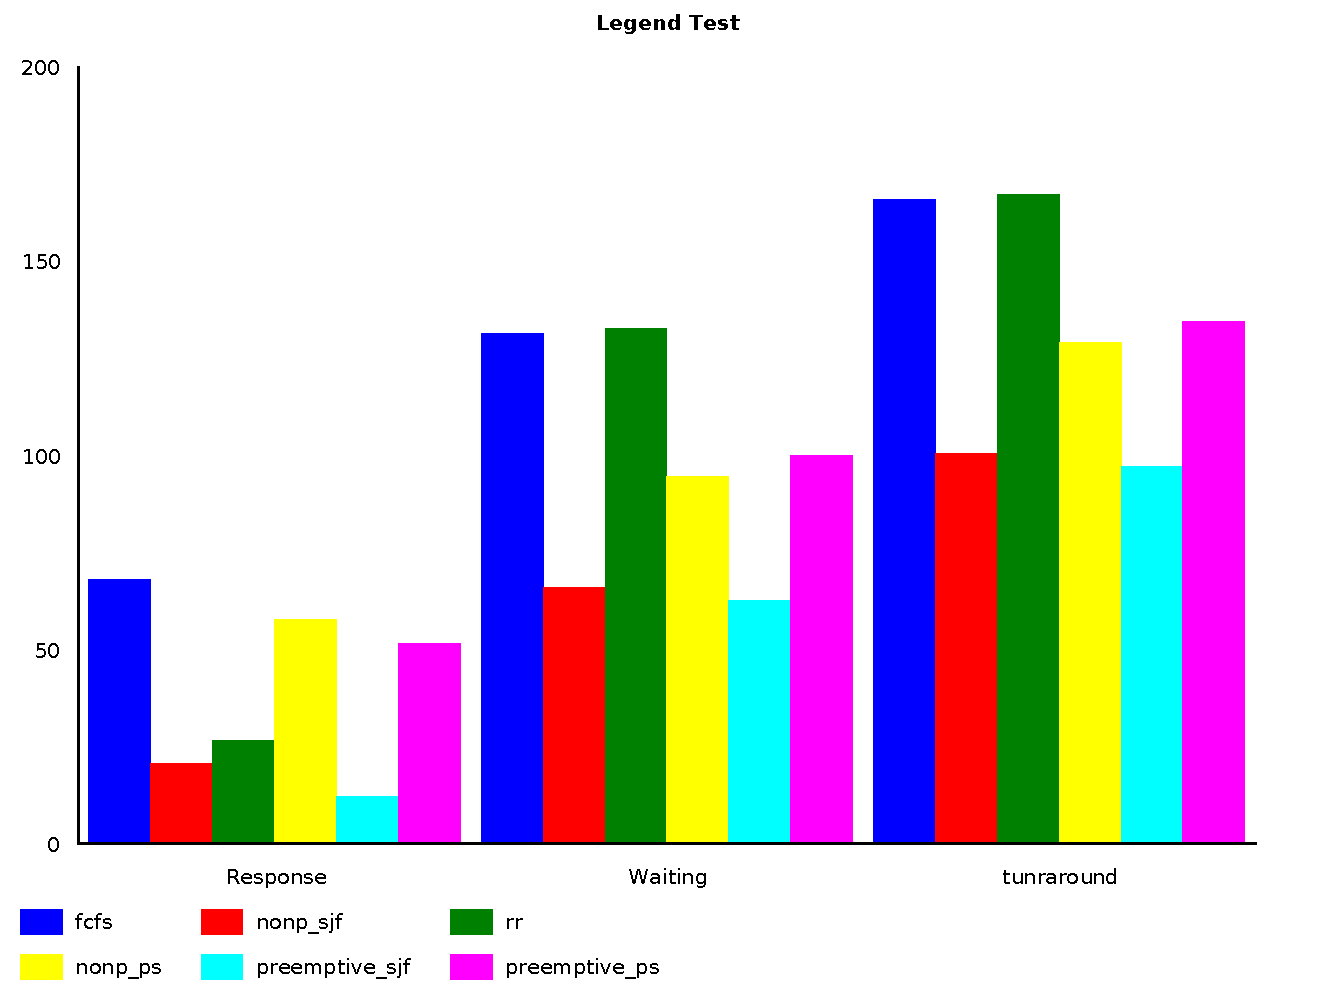
\includegraphics[scale=1]{averages}}
\caption{{\it Averages . Preemptive sjf clearly perform better than others . Round robin has a good response time}}  
\label{surf}
\end{figure} 
Then we have shown the comparison of average response .waiting and turnaround times for three priority categories 
\begin{figure}[ht]
\centerline{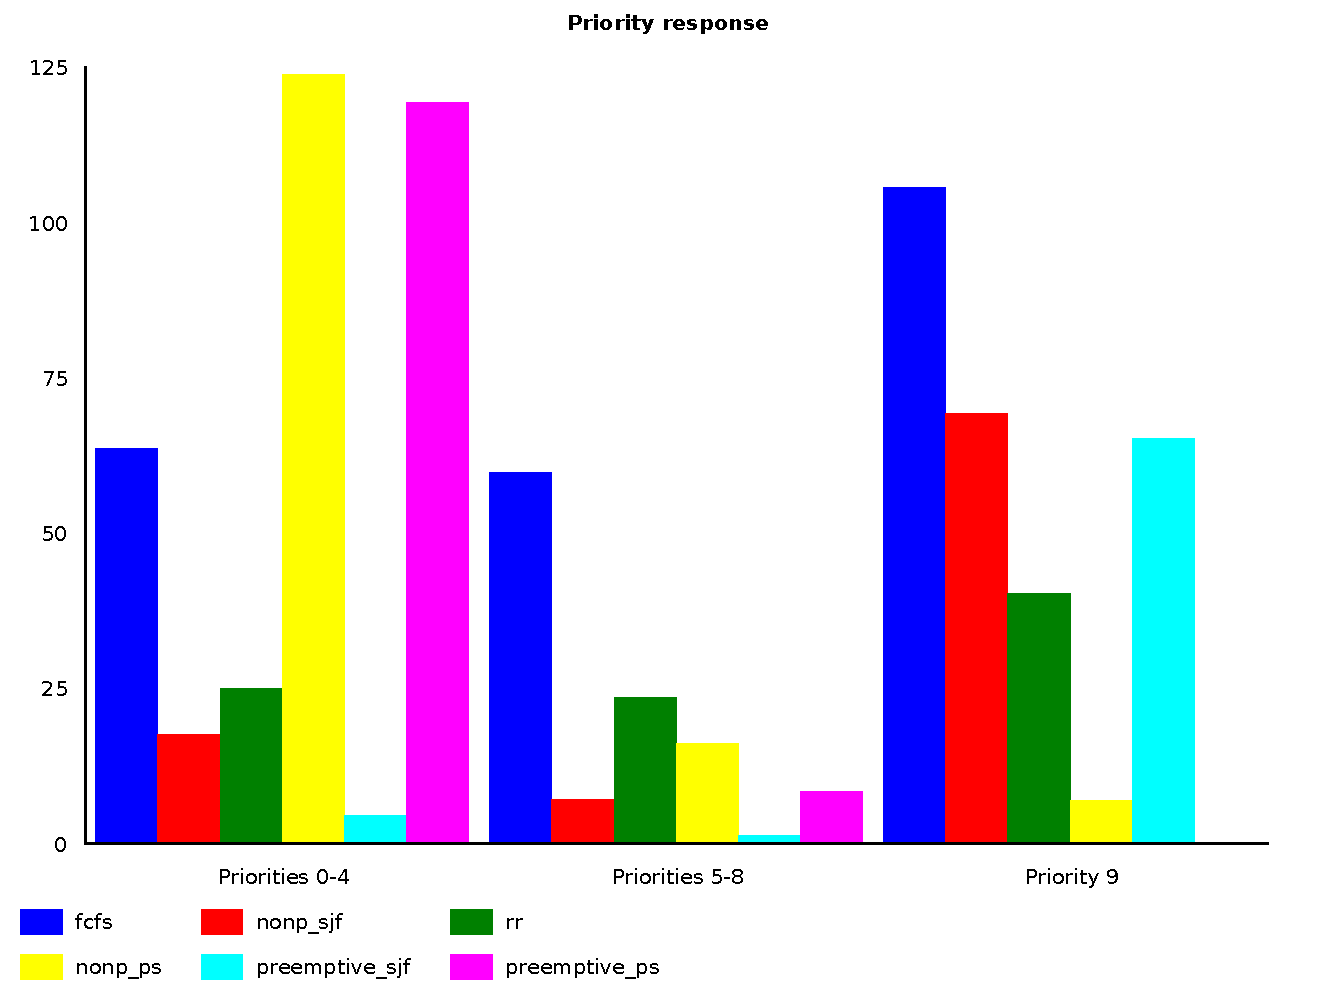
\includegraphics[scale=1]{priority_response_averages}}
\caption{{\it Average Response time . It can be clearly seen that the average response time for priority 9 is zero for preemptive priority scheduling}}  
\label{surf}
\end{figure}
\begin{figure}[ht]
\centerline{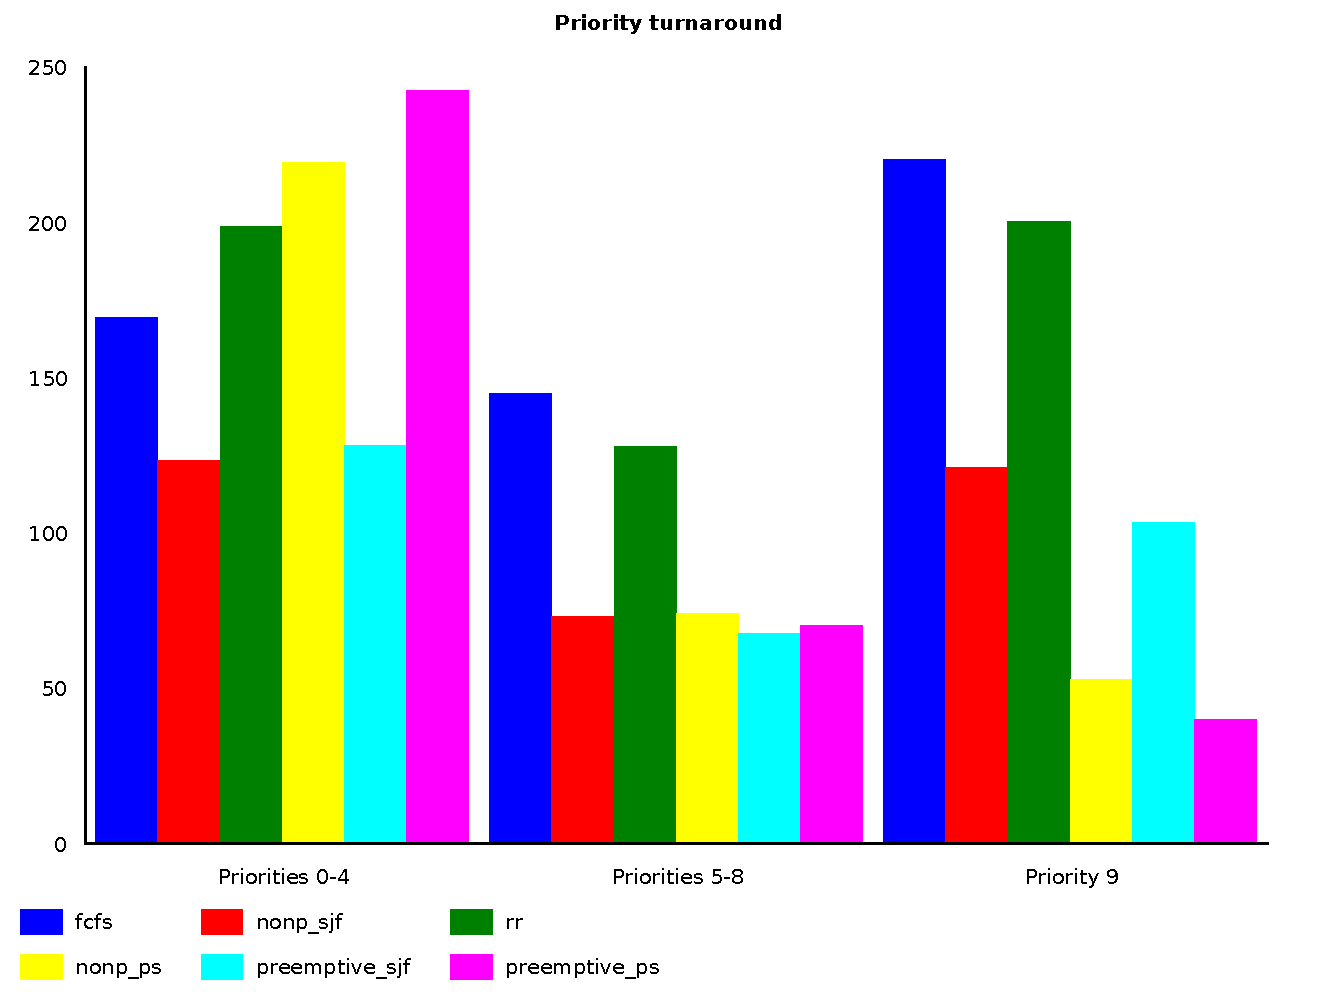
\includegraphics[scale=1]{priority_turnaround_averages}}
\caption{{\it Average turnaround time. Again preemptive priority scheduling for priority 9 beats other}}  
\label{surf}
\end{figure}
\begin{figure}[ht]
\centerline{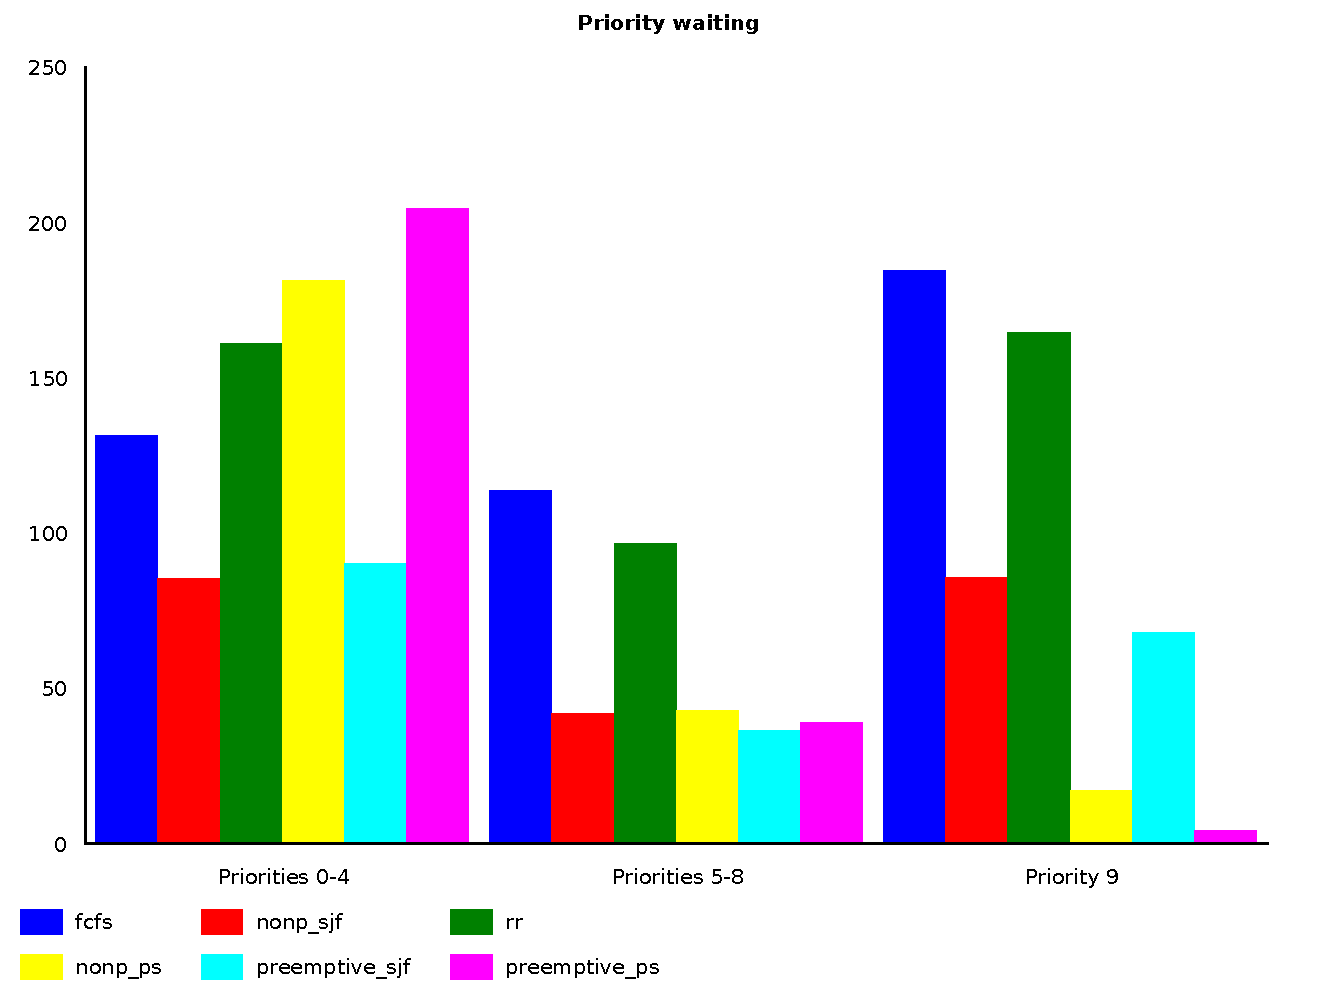
\includegraphics[scale=1]{priority_waiting_averages}}
\caption{{\it Average waiting time}}  
\label{surf}
\end{figure}

\section*{NACH OS}

\begin{itemize}
\item Our system can run upto 16 threads at the same time without crashing.Thereafter the behaviour is erratic as documented in the source code. 
\item The kernel is made preemptive by using timer interrupts every 100 ticks. Every 100 ticks , Alarm::CallBack(), our timer interrupt handler is called.
\item The main thread must have a response time of 0. There after the minimum response time is 10 ms due to context switching. Process with priority 9 is guaranteed to have a response time of 10 ms.
\item Our implementation consists of multi level queues , highQueue for priority 9 process , midQueue for process between priority 5 and 8 , and the lower priority processes are put in lowQueue.
\item Excluding the time spent in servicing priority 9 processes , the cpu spends 80 percent time in mid queue and 20 percent time in low queue.
\item This and rr scheduling guarantees that mid queue processes will have a finite response time.
\item The idea of cpu time division between mid and low queues makes the scheduler realistic and saves the low priority processes from starvation.
\end{itemize}
\section*{STATS}
\begin{itemize}
\item Thread Name : child
TotalTicks : 261
PID : 4
Priority : 7
Burst Time : 38
Arrival Time : 213
Response Time : 10
Waiting Time : 10
Turnaround Time : 48

Thread Name : main
TotalTicks : 310
PID : 0
Priority : -1
Burst Time : 138
Arrival Time : 0
Response Time : 0
Waiting Time : 172
Turnaround Time : 310

Thread Name : child
TotalTicks : 586
PID : 2
Priority : 9
Burst Time : 170
Arrival Time : 35
Response Time : 10
Waiting Time : 10
Turnaround Time : 551

Thread Name : child
TotalTicks : 728
PID : 3
Priority : 4
Burst Time : 116
Arrival Time : 68
Response Time : 61
Waiting Time : 113
Turnaround Time : 660

Thread Name : child
TotalTicks : 951
PID : 5
Priority : 7
Burst Time : 96
Arrival Time : 548
Response Time : 38
Waiting Time : 258
Turnaround Time : 403

Thread Name : child
TotalTicks : 1051
PID : 6
Priority : 4
Burst Time : 96
Arrival Time : 638
Response Time : 41
Waiting Time : 79
Turnaround Time : 413

\item 
Thread Name : child
TotalTicks : 261
PID : 4
Priority : 9
Burst Time : 38
Arrival Time : 213
Response Time : 10
Waiting Time : 10
Turnaround Time : 48

Thread Name : main
TotalTicks : 310
PID : 0
Priority : -1
Burst Time : 138
Arrival Time : 0
Response Time : 0
Waiting Time : 172
Turnaround Time : 310

Thread Name : child
TotalTicks : 731
PID : 2
Priority : 1
Burst Time : 170
Arrival Time : 35
Response Time : 10
Waiting Time : 167
Turnaround Time : 696

Thread Name : child
TotalTicks : 752
PID : 3
Priority : 6
Burst Time : 136
Arrival Time : 68
Response Time : 10
Waiting Time : 114
Turnaround Time : 684

Thread Name : child
TotalTicks : 854
PID : 5
Priority : 2
Burst Time : 86
Arrival Time : 548
Response Time : 10
Waiting Time : 182
Turnaround Time : 306

Thread Name : child
TotalTicks : 954
PID : 6
Priority : 7
Burst Time : 86
Arrival Time : 641
Response Time : 10
Waiting Time : 10
Turnaround Time : 313

\item
Thread Name : child
TotalTicks : 261
PID : 4
Priority : 6
Burst Time : 38
Arrival Time : 213
Response Time : 10
Waiting Time : 10
Turnaround Time : 48

Thread Name : main
TotalTicks : 310
PID : 0
Priority : -1
Burst Time : 138
Arrival Time : 0
Response Time : 0
Waiting Time : 172
Turnaround Time : 310

Thread Name : child
TotalTicks : 731
PID : 2
Priority : 0
Burst Time : 170
Arrival Time : 35
Response Time : 10
Waiting Time : 167
Turnaround Time : 696

Thread Name : child
TotalTicks : 752
PID : 3
Priority : 3
Burst Time : 136
Arrival Time : 68
Response Time : 10
Waiting Time : 114
Turnaround Time : 684

Thread Name : child
TotalTicks : 854
PID : 5
Priority : 7
Burst Time : 86
Arrival Time : 548
Response Time : 10
Waiting Time : 182
Turnaround Time : 306

Thread Name : child
TotalTicks : 954
PID : 6
Priority : 9
Burst Time : 86
Arrival Time : 641
Response Time : 10
Waiting Time : 10
Turnaround Time : 313

\end{itemize}


\end{document}